%%%%%%%%%%%%%%%%%%%%%%%%%%%%%%%%%%%%%%%%%%%%%%%%%%%%%%%%%%%%%%%%%%%%%%%%
% Preamble
%%%%%%%%%%%%%%%%%%%%%%%%%%%%%%%%%%%%%%%%%%%%%%%%%%%%%%%%%%%%%%%%%%%%%%%%
\documentclass[11pt]{article}
%
% Packages and other includes
% Pagination
\usepackage[letterpaper, margin=1in]{geometry}
\usepackage{emptypage}
\usepackage{mhchem}
%
% Fonts
\usepackage[T1]{fontenc} % best for Western European languages
\usepackage{lmodern} % Latin Modern instead of CM
\usepackage{textcomp} % required to get special symbols
%
% Math
\usepackage{amsmath, amssymb}
\usepackage{braket}
%
% Graphics, floats, tables
\usepackage{graphicx, color, float, array}
%
% Hyperlinks
\usepackage{hyperref}
%
%
% Definitions and settings
% Paragraph indent and spacing
\setlength{\parskip}{0.4\baselineskip}
\setlength{\parindent}{0in}
%
%
% Title, authors, date
\title{\textbf{Midterm 2 Problems}}
%
%
%%%%%%%%%%%%%%%%%%%%%%%%%%%%%%%%%%%%%%%%%%%%%%%%%%%%%%%%%%%%%%%%%%%%%%%%
% Main document
%%%%%%%%%%%%%%%%%%%%%%%%%%%%%%%%%%%%%%%%%%%%%%%%%%%%%%%%%%%%%%%%%%%%%%%%
%

\begin{document}

\maketitle

1. (5 pts) \textbf{Van't Hoff Equation} Nitrosyl chloride ClNO(g) decomposes
into NO(g) and Cl$_2$(g). The unbalanced chemical equation is
\begin{center}
  \ce{ClNO(g) <=> NO(g) + Cl$_2$(g)}
\end{center}
Using the Van't Hoff equation
\begin{equation}
  \ln K = -\frac{\Delta H^\circ}{RT} + \frac{\Delta S^\circ}{R}
  \label{eqn:van_hoff}
\end{equation}
and the gas phase thermochemistry data, determine the following. Report
all results to 3 significant figures.

(a) Balance the chemical equation.

(b) At what temperature is the equilibrium constant $K$ greater than 1?

(c) At 25$^\circ$C, suppose the reaction is at equilibrium. The temperature
is increased. Describe the change in $K$ in terms of the thermodynamic
quantities. \textit{Hint:} Create a plot to illustrate the process.

\begin{table}[hbpt]
  \caption{Reported $\Delta H^\circ$ (kJ/mol) and $\Delta S^\circ$ (J/(mol K))}
  \centering
  \begin{tabular}{c|cc}
    & $\Delta H^\circ$ & $\Delta S^\circ$ \\
    \hline
    NO        &  90.29 & 210.76 \\
    ClNO      &  51.71 & 261.68 \\
    Cl$_2$    &  0.00 & 223.08
  \end{tabular}
\end{table}

\pagebreak

2. (6 pts) \textbf{Mixing of Ideal Gas} Assume ideal gas conditions. At 25$^\circ$C,
nitrogen dioxide NO$_2$(g) and dinitrogen tetraoxide N$_2$O$_4$(g) are
separated into equal 1L compartments, see Fig. \ref{fig:mix}. The initial pressures of the
NO$_2$(g) and N$_2$O$_4$(g) are both at 1.25 atm. The valve is then opened allowing
the gases to mix. Report all results to 2 significant figures.

\begin{figure}[hbpt]
  \centering
  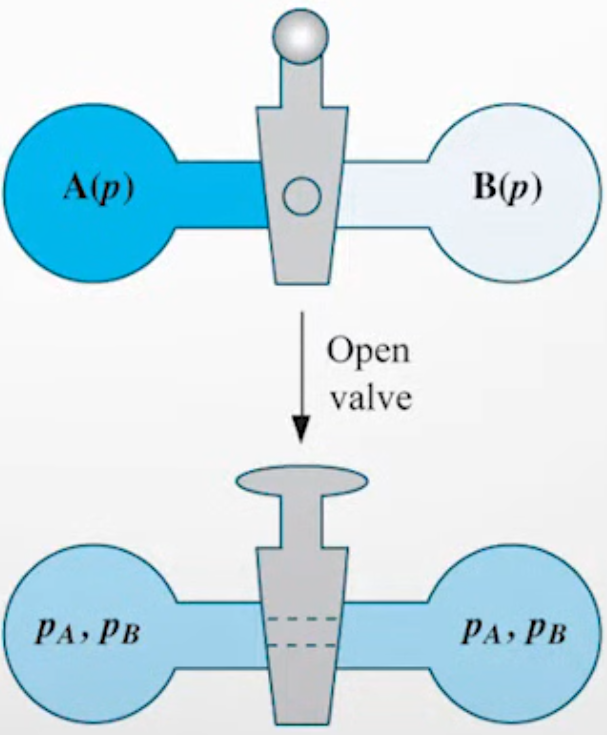
\includegraphics[scale=0.25]{mix_ideal.png}
  \caption{Illustration of gases A and B separated into equal volumes.}
  \label{fig:mix}
\end{figure}

(a) Determine the free energy of mixing $\Delta G_\text{mix}$ and entropy
of mixing $\Delta S_\text{mix}$.

(b) N$_2$O$_4$(g) is in equilibrium with NO$_2$(g). Write the balanced
chemical equation including states.

(c) At 25$^\circ$C, the equilibrium constant $K$ is 0.1481 for the N$_2$O$_4$(g)
decomposition. When the gases mix and allow to equilibrate, describe the ``driving
force'' in terms of the thermodynamic quantities.

% Free energy
% -81.670897 kJ/mol N2O2 and -38.467926 kJ/mol
% decomposition -> 4.735045 kJ/mol

\pagebreak

3. (4 pts) \textbf{Properties of Equilibrium Constants} Determine $K_c$ at 25$^\circ$C
for the reaction,
\begin{center}
  \ce{N$_2$(g) + O$_2$(g) + Cl$_2$(g) <=> 2 NOCl(g)},
\end{center}
given the following data set at 25$^\circ$C. Report result to 2 significant figures.
\begin{center}
  \ce{N$_2$(g) + 2 O$_2$(g) <=> 2 NO$_2$(g) $\,\,$ $K_p = 1.0\times 10^{-18}$}

  \ce{2 NOCl(g) + O$_2$(g) <=> 2 NO$_2$Cl(g) $\,\,$ $K_p = 1.21\times 10^4$}

  \ce{2 NO$_2$(g) + Cl$_2$(g) <=> 2 NO$_2$Cl(g) $\,\,$ $K_p = 9.0\times 10^{-2}$}
\end{center}

\pagebreak

\end{document}
